\documentclass[conference]{IEEEtran}

\IEEEoverridecommandlockouts

\usepackage{cite}
\usepackage{amsmath,amssymb,amsfonts}
\usepackage{graphicx}
\usepackage{textcomp}
\usepackage{xcolor}
\usepackage{array}
\usepackage{booktabs}
\usepackage{url}
\usepackage{tikz}
\usepackage{float}
\usetikzlibrary{shapes.geometric, arrows.meta, positioning}

\tikzstyle{process} = [
    rectangle,
    rounded corners=15pt,
    minimum width=4cm,
    minimum height=1cm,
    text centered,
    align=center,
    draw=black,
    fill=gray!10
]

\tikzstyle{decision} = [
    diamond,
    aspect=2,
    minimum width=4cm,
    minimum height=2cm,
    text centered,
    align=center,
    draw=black,
    fill=gray!10
]

\tikzset{
    >={Stealth[length=4mm,width=4mm]}
}

\tikzstyle{arrow} = [
    thick,
    ->,
    draw=black
]

\begin{document}

\title{AirSketch: A Gesture-Based Virtual Drawing System via MediaPipe}

\author{
\IEEEauthorblockN{
Dr. Anita Harsoor,
Hisham Khuram,
Md Ahmed Raza Sofi,
Mohammad Abdul Maaz Hanan
}

\IEEEauthorblockA{
Department of Computer Science and Engineering\\
P.D.A College of Engineering\\
Kalaburagi, India\\
\{anitaharsoor, 3pd23cs050, 3pd23cs065, 3pd23cs070\}@pdaengg.com
}
}

\maketitle

\begin{abstract}
AirSketch is an innovative interactive web application designed to transform the way users create digital drawings by leveraging real-time hand gesture recognition through a webcam. Instead of relying on traditional input devices such as a mouse, stylus, or touchscreen, the system interprets natural hand and finger movements and converts them into precise drawing actions on a virtual canvas.

By extending a single finger, users can draw seamlessly, while predefined gestures allow them to switch colors, activate eraser mode, or clear the canvas entirely, ensuring an intuitive and fluid user experience. The application integrates computer vision techniques to accurately track hand landmarks and maintain responsiveness, resulting in smooth and lag-free interaction.

AirSketch significantly improves accessibility by empowering physically challenged individuals to interact with digital systems using simple gestures, reducing dependency on conventional hardware. The system employs MediaPipe Hands for landmark detection, TensorFlow.js as the underlying ML runtime, and React with TypeScript for a responsive user interface. Experimental results confirm real-time frame processing at approximately 30 fps on standard hardware.

This project demonstrates the practical application of gesture-based interfaces in modern web technologies, offering a touch-free, efficient, and inclusive approach to digital drawing and human-computer interaction.
\end{abstract}

\begin{IEEEkeywords}
Hand gesture recognition, MediaPipe, TensorFlow.js, virtual drawing, human-computer interaction, computer vision, touchless interface, accessibility
\end{IEEEkeywords}

\section{Introduction}

Hand gesture recognition is one of the most widely studied approaches in the field of Human-Computer Interaction (HCI). By detecting and analyzing the movement and position of fingers and hands, computer systems can interpret specific gestures as commands. This technology has been applied across a broad spectrum of applications including virtual reality environments, interactive gaming systems, smart classrooms, sign language recognition, and touchless control interfaces~\cite{ref7}.

AirSketch presents a web-based interactive application that enables users to draw on a digital canvas solely through hand gestures captured by a standard webcam. The system tracks hand movements in real time, identifies specific finger configurations, and translates these gestures into drawing actions. Being entirely browser-native, it requires no specialized hardware beyond an integrated or USB webcam.

The motivation behind AirSketch stems from the increasing demand for touchless and inclusive HCI systems. Advancements in real-time computer vision and machine learning frameworks—particularly MediaPipe~\cite{ref3} and TensorFlow.js~\cite{ref10}—have made it feasible to build accurate, low-latency gesture recognition systems that operate entirely within a modern web browser.

\section{Related Work}

A comprehensive review of existing research in hand gesture recognition and virtual drawing systems was conducted to identify key technologies, methodologies, and limitations.

Chang et al.~\cite{ref1} introduce OMG-Bench, a large-scale dataset for skeleton-based online micro-gesture recognition. Moreira~\cite{ref2} proposes a CNN-based approach using spatiotemporal matrix representation for dynamic LIBRAS gesture recognition.

Vasavi et al.~\cite{ref3} present a gesture-driven virtual painting system using MediaPipe, enabling real-time hand tracking and intuitive drawing without physical contact. Swathi~\cite{ref4} describes an Air Canvas system using hand tracking for virtual drawing.

Mahmud et al.~\cite{ref5} propose a deep learning-based multimodal depth-aware system for dynamic gesture recognition. Sharma et al.~\cite{ref6} present a gesture recognition system leveraging image processing and contour-based feature extraction.

Qi et al.~\cite{ref7} provide a survey of computer vision-based hand gesture recognition methods for human-robot interaction. Morajkar et al.~\cite{ref8} combine hand gestures and voice commands for computer mouse control.

Anithadevi et al.~\cite{ref9} propose a MediaPipe-LSTM framework for real-time sign language recognition. Quan et al.~\cite{ref10} investigate faults in JavaScript-based deep learning systems.

Several researchers emphasize the use of computer vision and deep learning techniques for improving gesture recognition accuracy, responsiveness, and real-time interaction capabilities. MediaPipe-based approaches discussed in~\cite{ref3} and~\cite{ref9} show that lightweight hand tracking frameworks can achieve efficient landmark detection while maintaining low computational overhead, making them suitable for browser-based applications such as AirSketch.

The literature also highlights several practical challenges associated with gesture recognition systems, including lighting sensitivity, background noise, motion blur, and hand occlusion issues. While deep learning and multimodal approaches proposed in~\cite{ref2} and~\cite{ref5} improve recognition performance, they often require higher computational resources and specialized hardware. In contrast, webcam-based computer vision systems provide a more accessible and cost-effective solution for real-time virtual interaction. 

\section{Problem Statement and Objectives}

Traditional digital drawing systems rely on physical input devices such as a mouse, stylus, or touchscreen. These modalities require direct physical interaction that may be unintuitive, non-portable, or inaccessible for users with physical disabilities.

The AirSketch system is designed to develop a gesture-based virtual drawing platform capable of detecting and interpreting hand gestures in real time. The project aims to demonstrate AI-driven human-computer interaction using standard webcam hardware, eliminating the need for traditional input devices such as a mouse or stylus. In addition, the system seeks to enhance accessibility for users with physical limitations by enabling touch-free interaction.

The platform also provides an interactive interface with features such as virtual drawing, color selection, brush size adjustment, eraser mode, and canvas clearing functionality. Furthermore, the project focuses on creating a lightweight web-based solution that operates without requiring any specialized hardware, making the system cost-effective, portable, and easy to use.

Unlike conventional hardware-dependent gesture recognition systems, AirSketch operates entirely within a modern web browser and does not require external sensors or dedicated controllers. The project demonstrates how lightweight computer vision frameworks such as MediaPipe and browser-based technologies can be effectively integrated to create practical, real-time, and touchless interactive systems for modern digital environments.

\section{Existing Systems}

\subsection{Microsoft Kinect}

Microsoft Kinect is a motion-sensing system that employs RGB cameras, depth sensors, and infrared technology to track body movements including hand gestures~\cite{ref7}. The system was originally developed for gaming and interactive applications, but it later found applications in virtual reality, rehabilitation systems, education, and gesture-controlled environments. Kinect enables users to interact with digital systems without physical controllers by converting body and hand movements into digital commands.

However, Kinect requires specialized hardware and has limited portability. The dependency on external sensors increases system cost and setup complexity, making it less suitable for lightweight and browser-based applications. In addition, Kinect systems require sufficient physical space and controlled environmental conditions for accurate gesture tracking and interaction.

\subsection{Leap Motion Controller}

The Leap Motion Controller uses infrared cameras and optical sensors to capture precise hand and finger movements~\cite{ref5}. The device is capable of detecting fine-grained finger motion with high accuracy, making it suitable for applications such as virtual reality, 3D modeling, simulation systems, and gesture-controlled interfaces. Its ability to track finger orientation and movement in real time provides a highly interactive user experience.

Although highly accurate, the Leap Motion Controller depends on dedicated external hardware. The system requires proper calibration and positioning for effective gesture recognition, while its limited interaction range may reduce flexibility in practical environments. The requirement of specialized hardware also increases overall cost and limits accessibility for general users compared to webcam-based systems such as AirSketch.

\subsection{Comparative Analysis}

\begin{table}[h]
\caption{Comparison of Existing Systems and AirSketch}
\centering
\renewcommand{\arraystretch}{1.3}
\begin{tabular}{|p{1.8cm}|p{1.5cm}|p{1.7cm}|p{1.7cm}|}
\hline
\textbf{Feature} & \textbf{Kinect} & \textbf{Leap Motion} & \textbf{AirSketch} \\
\hline
Hardware & Specialized & Specialized & Webcam Only \\
\hline
Cost & High & High & Low \\
\hline
Portability & Low & Low & High \\
\hline
Platform & Desktop & Desktop/VR & Web Browser \\
\hline
Accessibility & Moderate & Moderate & High \\
\hline
Setup & Complex & Moderate & None \\
\hline
\end{tabular}
\end{table}

The comparison shows that most traditional gesture recognition systems rely on dedicated hardware and complex setup procedures, increasing cost and reducing portability. In contrast, AirSketch provides a lightweight and accessible solution by using standard webcam hardware and browser-based technologies. This makes the proposed system more practical for real-time gesture-controlled drawing applications and improves accessibility for a wider range of users.

\section{Proposed System}

AirSketch is a fully web-based application that enables users to draw on a digital canvas using real-time hand gestures captured through a webcam. The system combines computer vision, hand landmark detection, and gesture recognition techniques to create a touchless and interactive drawing environment. By eliminating the dependency on traditional input devices such as a mouse, stylus, or touchscreen, the application provides a more natural and intuitive approach to digital interaction.

The platform provides multiple interactive features to enhance the virtual drawing experience. Users can select colors through predefined hand gestures, adjust brush size dynamically, switch to eraser mode for correction, and clear the entire canvas using specific gestures. These functionalities enable a smooth and intuitive touch-free drawing interface. The system continuously tracks fingertip movement and converts it into drawing strokes on the virtual canvas, allowing users to create digital sketches in real time.

Real-time processing ensures that user movements are instantly reflected on the screen, creating a smooth and natural drawing experience. The system processes webcam frames at a high frame rate, enabling low-latency gesture detection and rendering. MediaPipe hand tracking technology is used to accurately identify hand landmarks and finger positions, while browser-based processing ensures efficient performance without requiring additional software installation.

Additionally, AirSketch promotes accessibility by enabling touchless interaction, making it especially useful for individuals with physical disabilities or hand mobility limitations. The system also reduces dependency on expensive hardware-based gesture recognition systems by using only a standard webcam for operation.

Overall, AirSketch offers a cost-effective, accessible, and intuitive solution that enhances human-computer interaction through gesture-based control. The project further demonstrates the practical implementation of modern computer vision technologies in creating responsive, real-time, and user-friendly interactive systems for education, creativity, and assistive applications.

\section{Methodology}

\subsection{Video Input and Data Capture}
The system begins by capturing real-time video input through the user's webcam using browser-
native APIs. The continuous video stream is divided into individual frames, each of which is
analyzed using computer vision techniques to detect the presence of a hand and extract relevant
visual information. Frames are processed at each animation cycle to maintain real-time
responsiveness.

The webcam module continuously streams frames to the processing pipeline with minimal delay,
ensuring smooth interaction between the user and the application. Since the system operates
entirely within a web browser, video acquisition is handled efficiently without requiring external
software or additional device drivers.

\subsection{Hand Detection and Landmark Extraction}

Once a frame is captured, the MediaPipe Hands library is applied to detect hand presence and extract
21 key hand landmarks in 3D space. These landmarks correspond to anatomical positions on the
hand, including fingertips, knuckles, and the palm base. The landmark positions are normalized
relative to the frame dimensions, enabling consistent detection across different camera resolutions
and user distances.

MediaPipe utilizes machine learning and computer vision techniques to provide accurate and
efficient hand landmark tracking in real time. This improves gesture recognition accuracy and maintains smooth
tracking performance during continuous motion.

\subsection{Gesture Recognition}

Based on the position and relative configuration of hand landmarks, the system classifies specific
gestures. A single extended index finger triggers the drawing mode, mapping fingertip coordinates
directly onto the canvas. Other finger configurations — such as pinching or multiple extended
fingers — activate tool-switching gestures for color selection, eraser mode, or canvas clearing.

The gesture recognition process focuses on identifying predefined finger states and fingertip
relationships to ensure reliable interaction. This lightweight approach improves responsiveness while reducing computational
requirements for real-time browser-based execution.

\subsection{Drawing and Canvas Rendering}

The detected fingertip coordinates are mapped onto the HTML5 Canvas element to generate drawing
strokes in real time. Consecutive fingertip positions are connected using smooth Bezier curve
interpolation to render fluid, natural-looking strokes. The canvas maintains a persistent drawing
state, enabling users to build complex compositions across multiple gestures. Tool parameters such
as color and brush size are stored in application state and applied to each new stroke.

The rendering engine continuously updates the virtual canvas as new gesture data is received,
ensuring immediate visual feedback for user movements. Brush thickness, stroke color, and eraser
operations are dynamically applied during drawing, providing an interactive and realistic digital
sketching experience. Real-time rendering also minimizes delay between gesture input and screen
output, improving usability and responsiveness.

\subsection{Technical Stack}

The AirSketch system is implemented using modern web technologies and browser-based machine
learning frameworks to achieve lightweight and efficient real-time performance.

\begin{itemize}
    \item React 18 + TypeScript
    \item MediaPipe Hands
    \item TensorFlow.js
    \item Vite
    \item Tailwind CSS
\end{itemize}

\subsection{System Architecture Overview}

The system follows a pipeline architecture: Webcam Input → Frame Capture → MediaPipe
Landmark Detection → Gesture Classification → Canvas Rendering. Each stage is optimized for
minimal latency, ensuring the user perceives drawing as a direct extension of their hand movement.

The modular architecture allows different processing stages to operate efficiently and independently,
improving maintainability and scalability of the system. This architecture enables AirSketch to provide a
responsive and intuitive gesture-controlled drawing experience using only standard webcam
hardware.

\begin{figure*}[t]
\centering

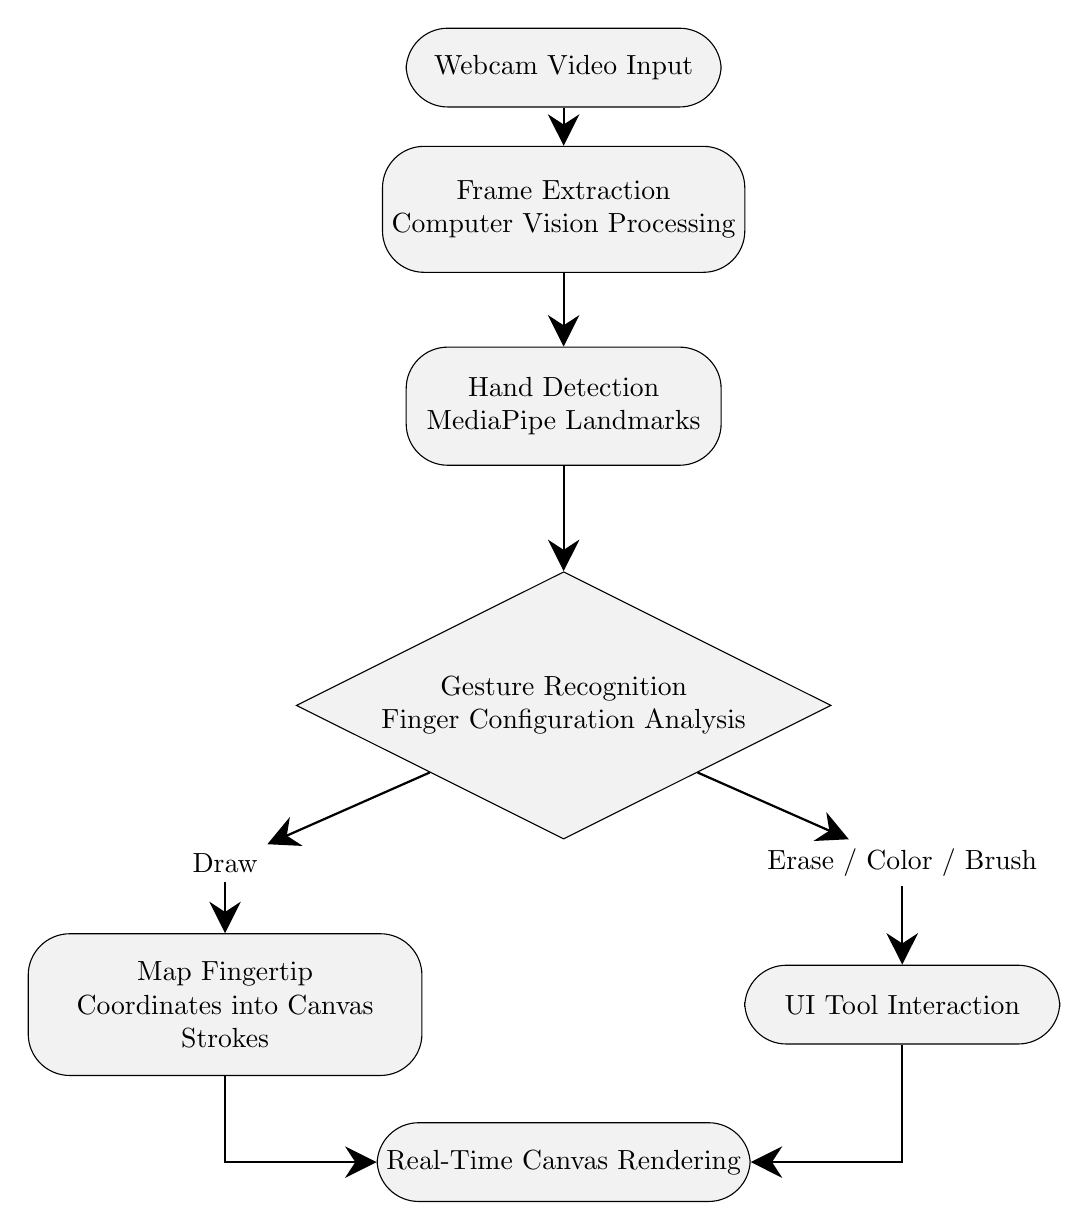
\begin{tikzpicture}[node distance=1.8cm]

% Nodes
\node (input) [process] {Webcam Video Input};

\node (frame) [process, below of=input, minimum height=1.6cm] 
{Frame Extraction\\Computer Vision Processing};

\node (hand) [process, below of=frame, minimum height=1.5cm, yshift=-0.7cm] 
{Hand Detection\\MediaPipe Landmarks};

\node (gesture) [decision, below of=hand, yshift=-2cm] 
{Gesture Recognition\\Finger Configuration Analysis};

\node (drawlabel) [left of=gesture, xshift=-2.5cm, yshift=-2cm] {Draw};

\node (toollabel) [right of=gesture, xshift=2.5cm, yshift=-2cm] 
{Erase / Color / Brush};

\node (draw) [process, below of=drawlabel, minimum width=5cm, minimum height=1.8cm] 
{Map Fingertip\\Coordinates into Canvas\\Strokes};

\node (tool) [process, below of=toollabel] 
{UI Tool Interaction};

\node (render) [process, below of=gesture, yshift=-4cm] 
{Real-Time Canvas Rendering};

% Arrows
\draw [arrow] (input) -- (frame);

\draw [arrow] (frame) -- (hand);

\draw [arrow] (hand) -- (gesture);

\draw [arrow] (gesture.south west) -- (drawlabel);

\draw [arrow] (gesture.south east) -- (toollabel);

\draw [arrow] (drawlabel) -- (draw);

\draw [arrow] (toollabel) -- (tool);

\draw [arrow] (draw.south) |- (render.west);

\draw [arrow] (tool.south) |- (render.east);

\end{tikzpicture}

\caption{Methodology flowchart of the AirSketch system.}
\label{fig:flowchart}

\end{figure*}

\section{Results and Discussion}

The AirSketch system was evaluated on laptops equipped with integrated 720p webcams running Chrome under Windows 11 and Ubuntu 22.04.

\begin{table}[h]
\caption{Performance Characteristics of AirSketch}
\centering
\renewcommand{\arraystretch}{1.3}
\begin{tabular}{|p{2.6cm}|p{1.5cm}|p{2.2cm}|}
\hline
\textbf{Performance Metric} & \textbf{Value} & \textbf{Condition} \\
\hline
Detection Rate & $\sim$30 fps & 720p Webcam \\
\hline
Latency & $<$50 ms & Indoor Lighting \\
\hline
Drawing Accuracy & $>$95\% & Index Finger Gesture \\
\hline
Memory Footprint & $<$150 MB & Chrome Browser \\
\hline
\end{tabular}
\end{table}

The AirSketch system demonstrates effective real-time gesture-based drawing functionality across standard hardware configurations. The application successfully detects hand landmarks using MediaPipe with low latency, enabling users to draw on the canvas in a smooth and responsive manner.

The core features including finger-tracking drawing, color selection, eraser mode, and canvas clearing all function correctly through predefined gesture configurations.

Key performance characteristics observed during implementation and testing include:

\begin{itemize}
    \item Low-latency landmark detection achieving real-time frame processing at approximately 30 frames per second on standard hardware.
    
    \item Accurate single-finger drawing mode enabling controlled and precise stroke creation.
    
    \item Robust gesture classification for tool-switching operations under normal indoor lighting conditions.
    
    \item Accessible browser-native deployment requiring no additional software installation beyond a modern web browser.
\end{itemize}

Challenges encountered include sensitivity to lighting variations and occasional landmark jitter,
which can cause minor stroke irregularities. Overall, the results validate
the feasibility and effectiveness of a lightweight, webcam-based gesture drawing system.

\begin{figure}[h]
\centering
\includegraphics[width=0.45\textwidth]{result1.png}
\caption{Real-time gesture-based drawing using AirSketch.}
\label{fig:drawing}
\end{figure}

\begin{figure}[h]
\centering
\includegraphics[width=0.45\textwidth]{result2.png}
\caption{The AirSketch canvas.}
\label{fig:tracking}
\end{figure}



\section{Conclusion}

This paper presents AirSketch, a web-based gesture-driven virtual drawing application leveraging MediaPipe hand tracking and TensorFlow.js for touchless interaction.

The implementation confirms that a lightweight webcam-based approach can deliver responsive gesture-based interaction while maintaining accessibility and low computational overhead.

Future enhancements include multi-hand support, undo/redo gestures, adaptive stroke smoothing, and cloud-based drawing storage.

\begin{thebibliography}{00}

\bibitem{ref1}
H. Chang et al., ``OMG-Bench: A New Challenging Benchmark for Skeleton-based Online Micro Hand Gesture Recognition,'' arXiv, 2026.

\bibitem{ref2}
J. Moreira, ``Dynamic LIBRAS Gesture Recognition via CNN over Spatiotemporal Matrix Representation,'' arXiv, 2026.

\bibitem{ref3}
R. Vasavi et al., ``Painting with Hand Gestures using MediaPipe,'' IJISRT, 2022.

\bibitem{ref4}
A. Swathi, ``Air Canvas Hand Tracking,'' JETIR, 2024.

\bibitem{ref5}
H. Mahmud et al., ``A Deep Learning-based Multimodal Depth-Aware Dynamic Hand Gesture Recognition System,'' ResearchGate, 2022.

\bibitem{ref6}
A. Sharma et al., ``Hand Gesture Recognition using Image Processing and Feature Extraction Techniques,'' ResearchGate, 2020.

\bibitem{ref7}
J. Qi et al., ``Computer Vision-based Hand Gesture Recognition for Human-Robot Interaction: A Review,'' SpringerNature, 2023.

\bibitem{ref8}
A. Morajkar et al., ``Hand Gesture and Voice-controlled Mouse for Physically Challenged using Computer Vision,'' ResearchGate, 2022.

\bibitem{ref9}
N. Anithadevi et al., ``MediaPipe-LSTM-Enhanced Framework for Real-Time Dynamic Sign Language Recognition,'' Wiley, 2024.

\bibitem{ref10}
L. Quan et al., ``Towards Understanding the Faults of JavaScript-Based Deep Learning Systems,'' arXiv, 2023.

\end{thebibliography}

\end{document}
